%%%%%%%%%%%%%%%%%%%%
%%%%% PREAMBLE %%%%%
%%%%%%%%%%%%%%%%%%%%

% Use the beamer class and configure it
\documentclass[aspectratio=169]{beamer}
\setbeamertemplate{section in toc}[square]
\setbeamertemplate{subsection in toc}[square]
\setbeamercolor{subsection in toc}{fg=alerted text.fg}
\setbeamercolor{subsection in toc shaded}{fg=structure}

% Use the metropolis theme and configure it
\usetheme
    [
      titleformat = smallcaps,
      numbering = fraction,
      progressbar = foot,
      block = fill
    ]
    {metropolis}

\usepackage[font={scriptsize,it}, labelfont={scriptsize,it}, justification=centering]{caption}
\usepackage{booktabs}
\usepackage{ragged2e}
\usepackage{pifont}

\definecolor{custom-red}{RGB}{225,99,92}
\definecolor{custom-green}{RGB}{119,193,108}

% Presentation main information
\title{Static Analysis Tool Exposition (SATE)\\Test Case Development}
\date{December 2\textsuperscript{nd}, 2016}
\author{\textbf{Damien Cupif}}
\institute{\textbf{\textit{Oral Defense for TELECOM Nancy Master's Degree}}}

% Include the table of contents at the beggining of each section
%% \AtBeginSection[]
%% {
%%   \begin{frame}
%%     \frametitle{Outline}
%%     \tableofcontents[currentsection]
%%   \end{frame}
%% }

% Include the table of contents at the beginning of each subsection
\AtBeginSubsection[]
{
  \begin{frame}[noframenumbering, plain]
    \frametitle{Outline}
    \tableofcontents[subsectionstyle=show/shaded/hide]
  \end{frame}
}

\newenvironment{changemargin}[2]{%
\begin{list}{}{%
\setlength{\topsep}{0pt}%
\setlength{\leftmargin}{#1}%
\setlength{\rightmargin}{#2}%
\setlength{\listparindent}{\parindent}%
\setlength{\itemindent}{\parindent}%
\setlength{\parsep}{\parskip}%
}%
\item[]}{\end{list}}

%%%%%%%%%%%%%%%%%%%%
%%%%% DOCUMENT %%%%%
%%%%%%%%%%%%%%%%%%%%

\begin{document}

  % Title frame
  \maketitle

  % Intro frames
  \section*{Introduction}
  
  \begin{frame}{About NIST}
    \begin{columns}[t]
      \begin{column}{0.29\textwidth}
        \begin{figure}
          \centering
          
\includegraphics[scale=0.14]{figures/nist-central-role}
          \caption{NIST, coordinating innovation since 1901}
        \end{figure}
      \end{column}
      \begin{column}{0.71\textwidth}
        \begin{small}
        \begin{itemize}
        \item US \textbf{N}ational \textbf{I}nstitute of \textbf{S}tandards and \textbf{T}echnology
        \item A non-regulatory agency in Dept. of Commerce
        \item \alert{+3,000} employees + adjuncts
        \item HQs in Gaithersburg, MD and Boulder, CO
        \item \textbf{Foster innovation by providing technology measurements and standards}
        \end{itemize}
        \end{small}
        \begin{figure}
          \centering
          
\includegraphics[scale=0.14]{figures/nist-logo}
          \caption{NIST Logo}
        \end{figure}
      \end{column}
    \end{columns}
  \end{frame}

  \begin{frame}{SAMATE Team}
    \begin{itemize}
    \setlength\itemsep{0.7em}
    \item \textbf{S}oftware \textbf{A}ssurance \textbf{M}etrics \textbf{A}nd \textbf{T}ool \textbf{E}valuation
    \item Team of \alert{about 10} software quality experts
    \item A strong focus on software security
    \item \textbf{Define software metrics and design best practices for evaluating software and security tools}
    \end{itemize}
    \begin{figure}
      \centering
      
\includegraphics[scale=0.4]{figures/samate-logo}
      \caption{SAMATE Logo}
    \end{figure}
  \end{frame}

  \begin{frame}{Low Level Structural Organization Chart}
    \begin{figure}
      \centering
      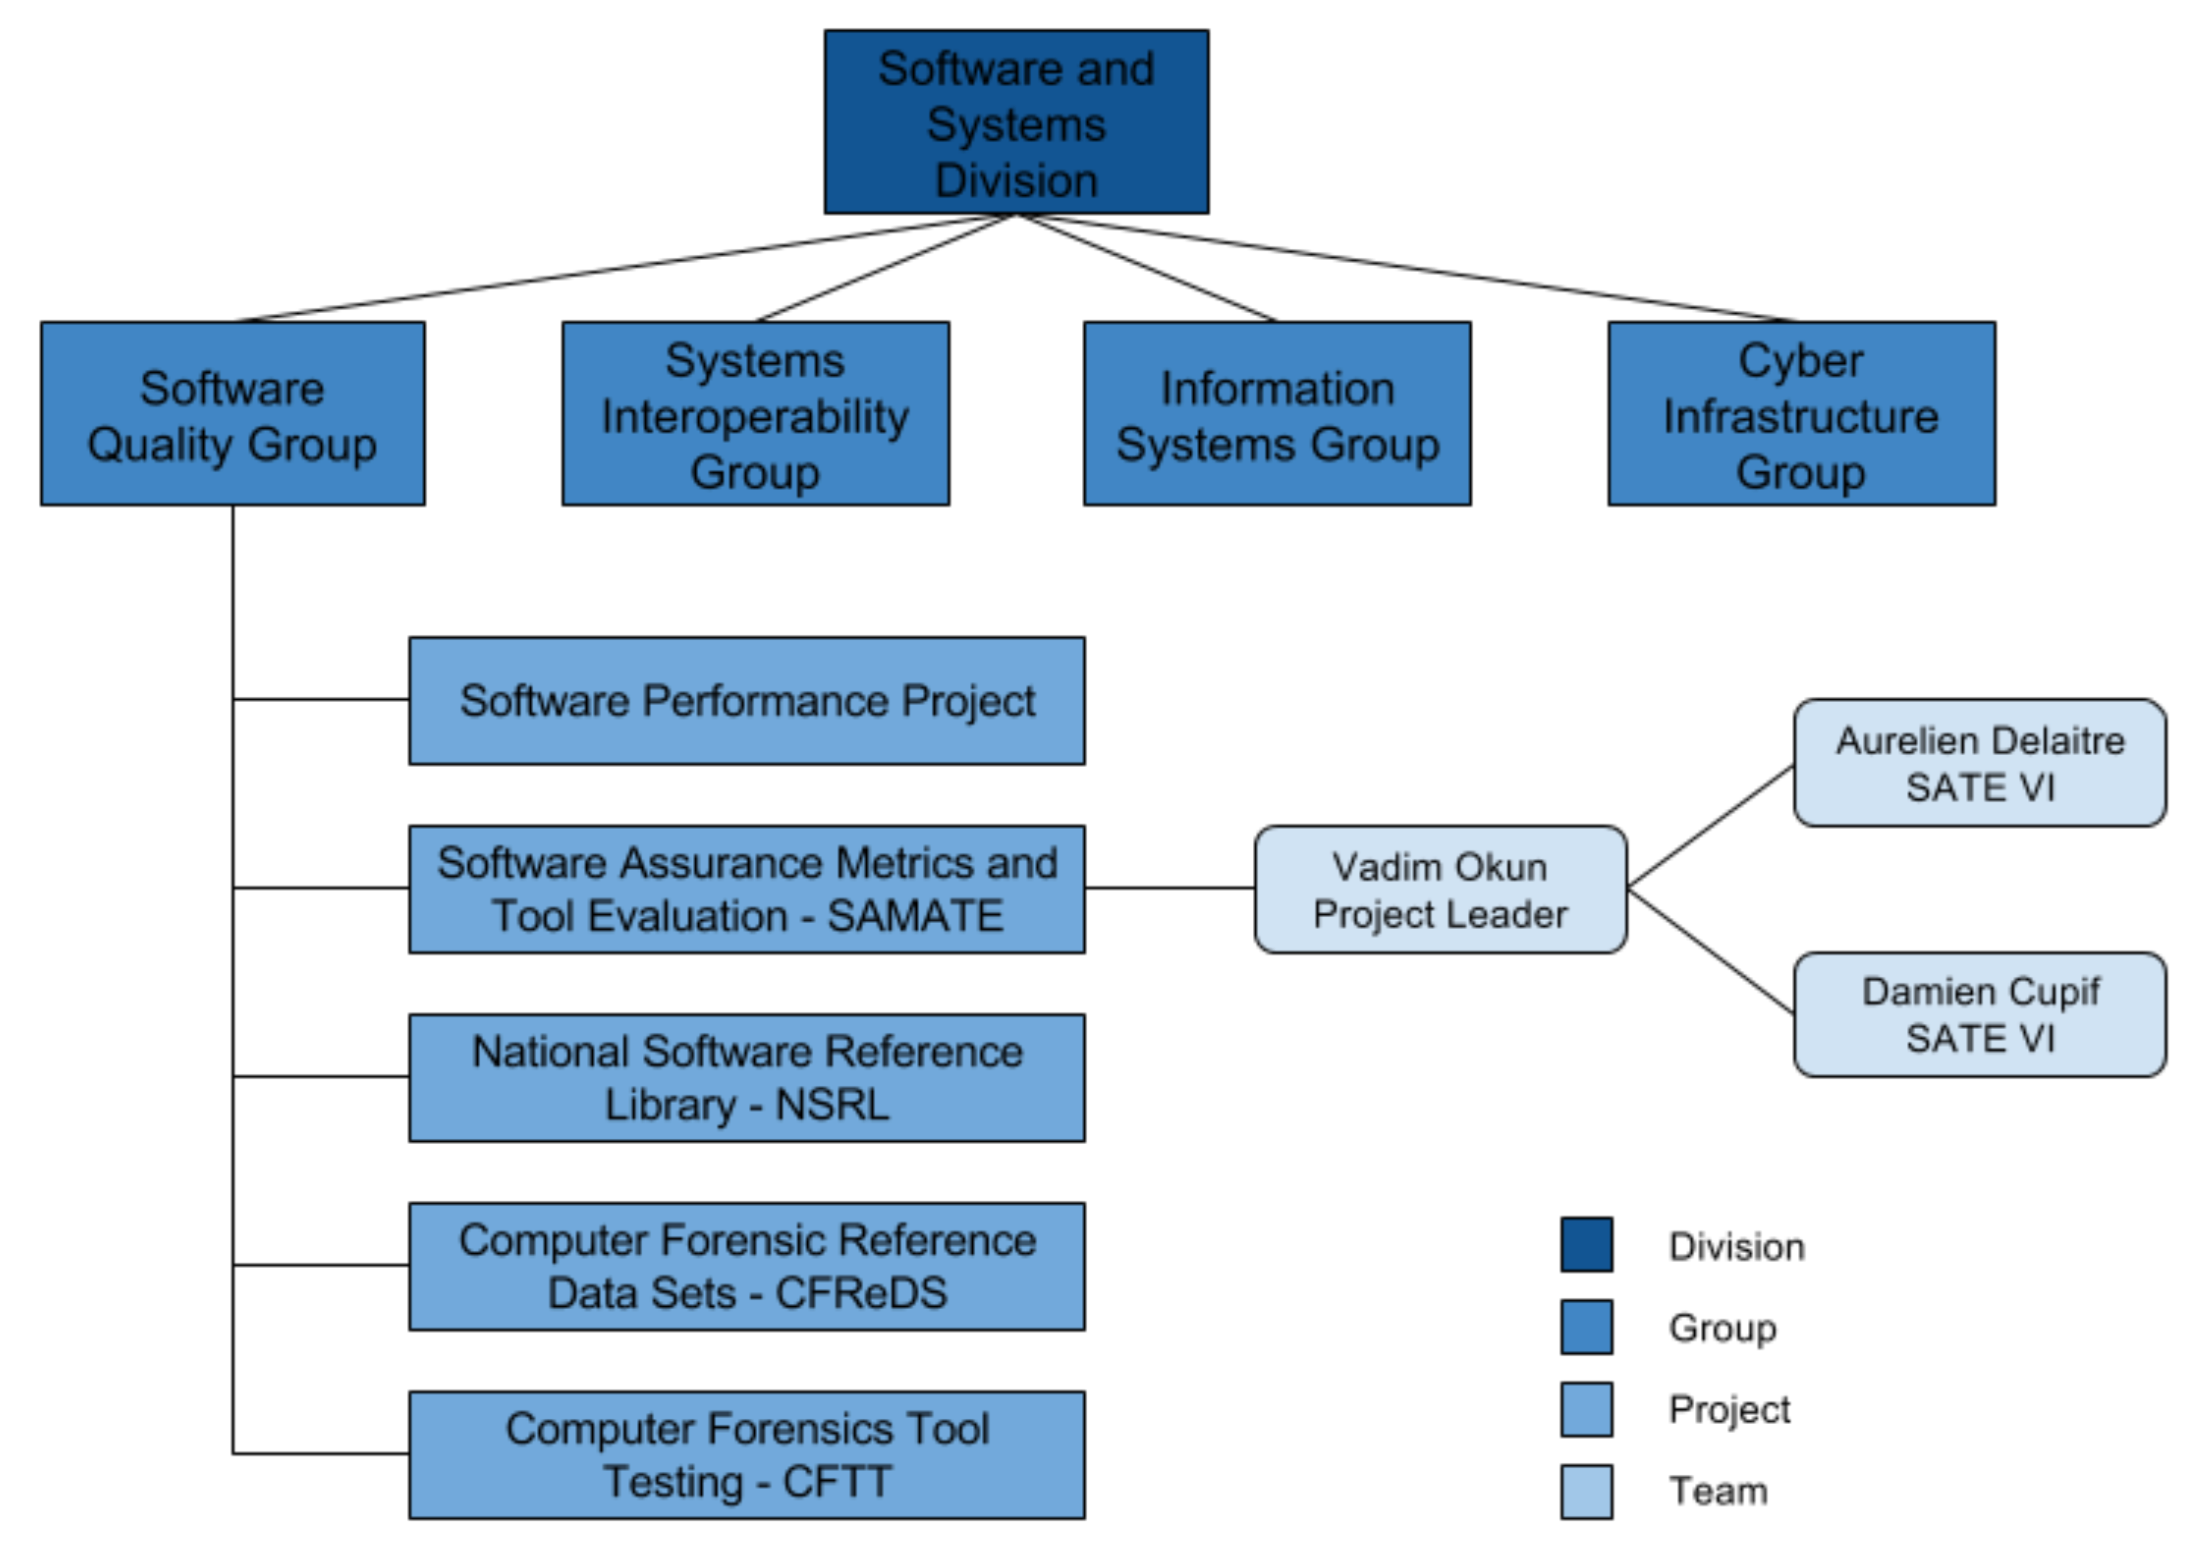
\includegraphics[scale=0.23]{figures/nist-division-organization-chart}
      \caption{Software and Systems Division Organization Chart}
    \end{figure}
  \end{frame}
  
  % Display fully the table of contents once
  \section*{Outline}
  \begin{frame}[noframenumbering, plain]{Outline}
    \tableofcontents[hideallsubsections]
  \end{frame}

  % Beginning of section
  \section{An Introduction to Static Analysis Tool Evaluation}
  
  \subsection{The Need for Software Assurance}
  
  \begin{frame}[standout]
    \begin{quote}
      `` Software is eating the world. ''\\
      --- Marc Andreessen
    \end{quote}
  \end{frame}
  
  \begin{frame}{General Facts About Software}
    \pause
    \begin{description}
      \item[Fact 1:] Software is \textbf{everywhere} and \textbf{powers critical infrastructures} in our everyday lives\\
    \end{description}
    \pause
    \begin{center}
    We trust software blindly, and yet \ldots
    \end{center}
    \vspace{-1.3em}
    \pause
    \begin{description}
      \vfill  
      \item[Fact 2:] Software has \textbf{bugs}
    \end{description}
    \pause
    \vfill
    \begin{definition}
      \vspace{0.3em}
      A \textcolor{mLightGreen}{bug} is a defect in a system that may or may not lead to its \textbf{unexpected behavior}.
    \end{definition}
    \vfill
  \end{frame}

  \begin{frame}{Is that a serious issue?}
    \vspace{0.5em}
    \begin{figure}
      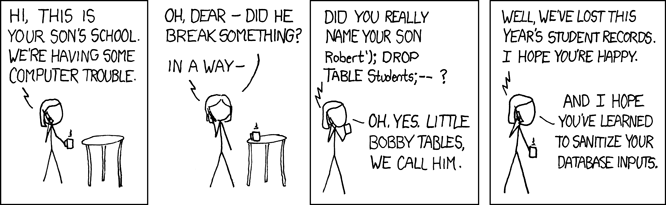
\includegraphics[scale=0.6]{figures/exploits_of_a_mom}
      \caption{Exploits of a Mom}
    \end{figure}
  \end{frame}
  
  \begin{frame}{What can we do?}
    \vspace{-1.4em}
    \begin{columns}[b]
      \begin{column}{0.5\textwidth}
        \begin{figure}
          \centering
          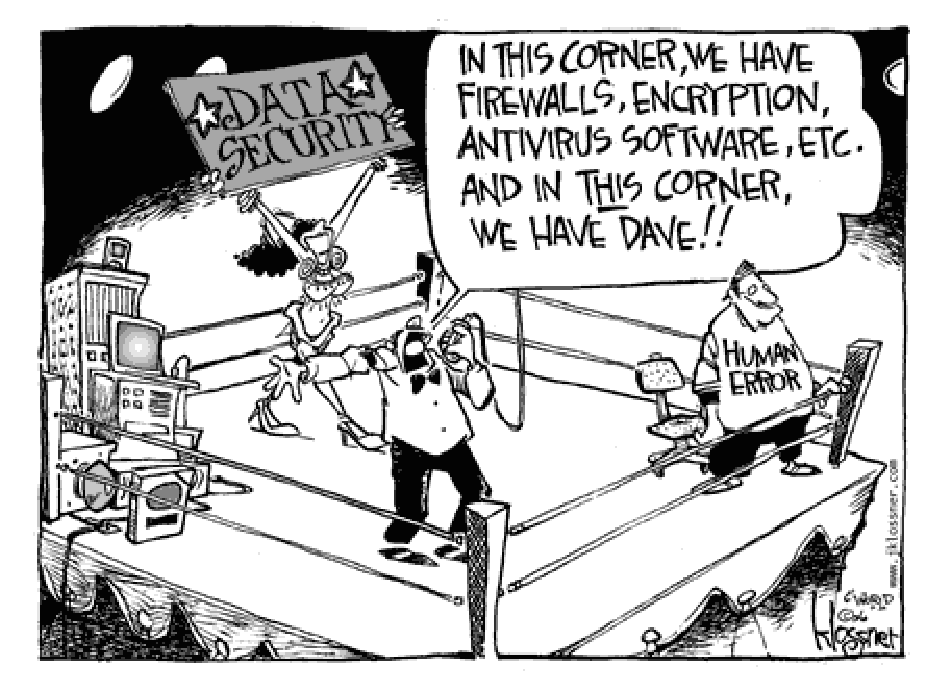
\includegraphics[scale=0.38]{figures/dave}
        \end{figure}
      \end{column}
      \begin{column}{0.5\textwidth}
        But wait \ldots{} we already have:
        \begin{itemize}
        \item firewalls
        \item antivirus software
        \item intrusion detection systems
        \item and more!
        \end{itemize}
        \pause
        Stop, \textbf{treating the symptoms} is not enough!
      \end{column}
    \end{columns}
    \centering
    \vfill
    \pause
    {\LARGE $\to$ We MUST build \alert{better software} in the first place!}
  \end{frame}

  \begin{frame}[standout]
    \begin{changemargin}{-2cm}{-2cm}
    \vspace{-0.2cm}
    \begin{figure}
      \centering
      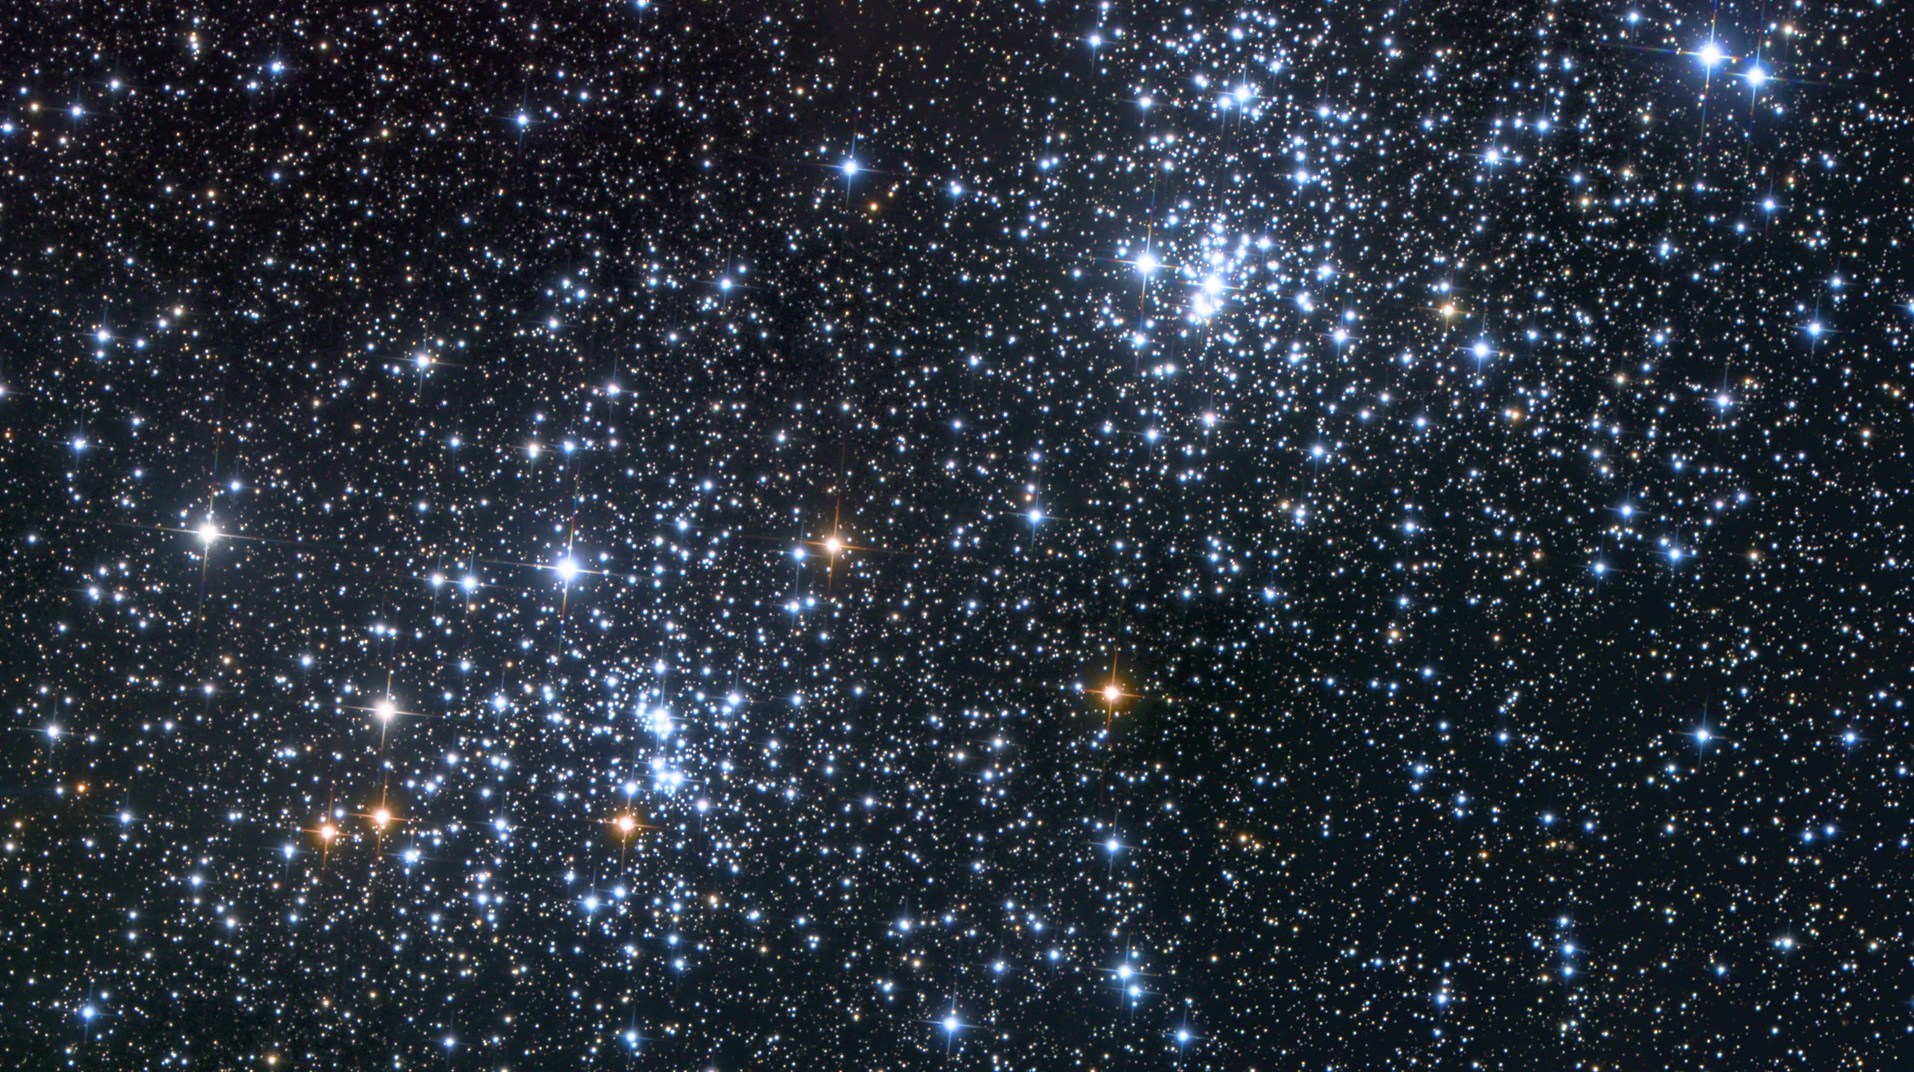
\includegraphics[scale=0.24]{figures/universe}
    \end{figure}
    \end{changemargin}
  \end{frame}

  \subsection{What is Static Analysis?}

  \begin{frame}{What is Static Analysis?}
    \begin{quote}
      \begin{flushright}
        ``The term \alert{static analysis} refers to any process\\ for assessing code \textbf{without executing it}''\\
        --- Brian Chess, Jacob West
      \end{flushright}
    \end{quote}
    \pause
    \begin{figure}
      \centering
      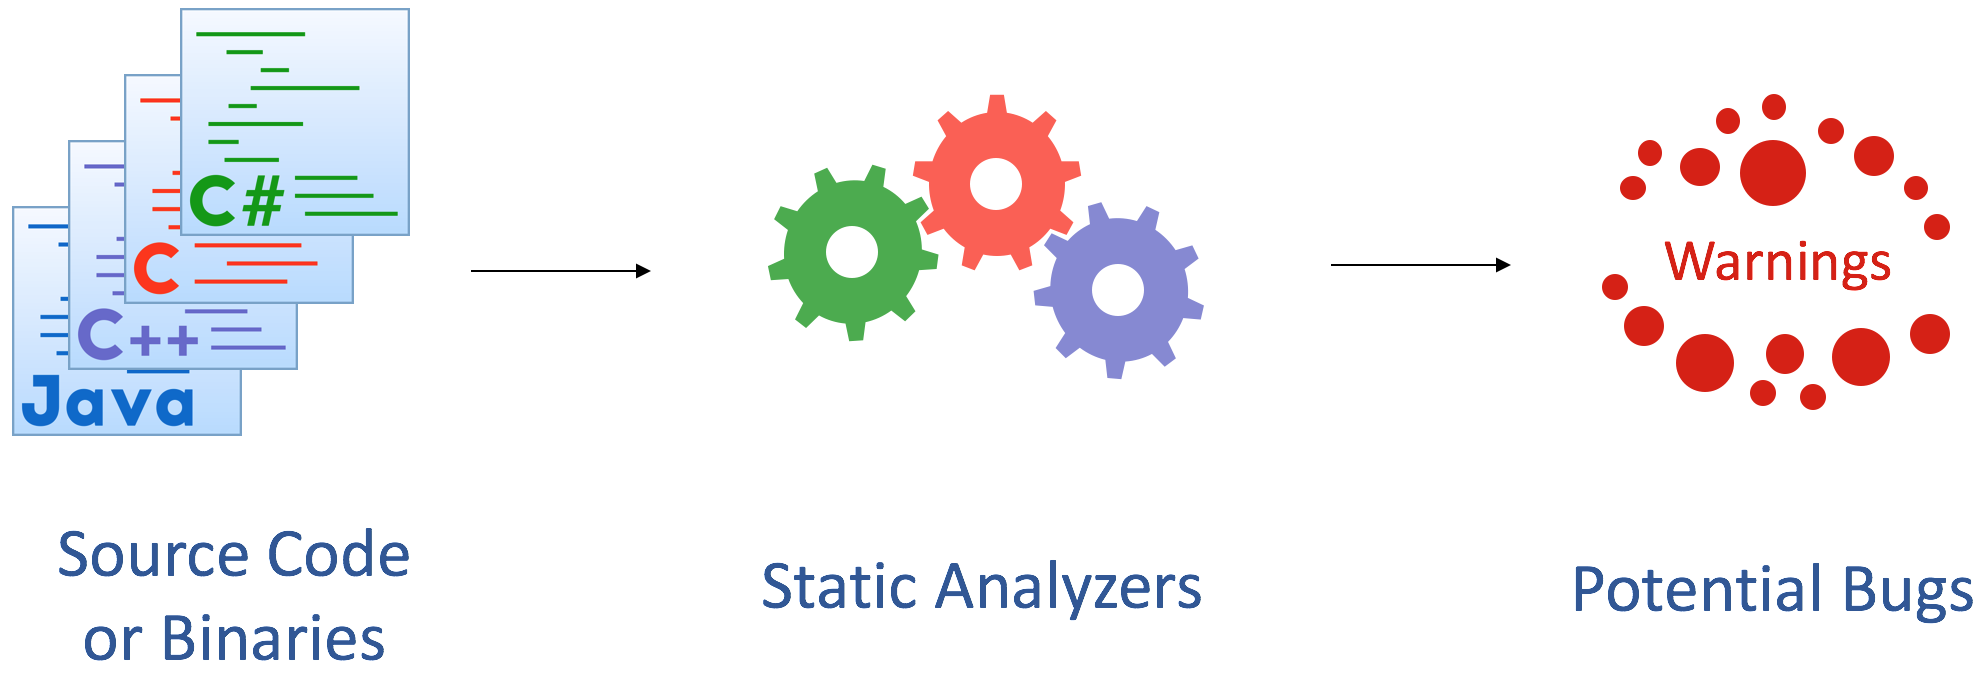
\includegraphics[scale=0.35]{figures/static-analysis}
      \caption{High Level Static Analysis Process Overview}
    \end{figure}
  \end{frame}

  \begin{frame}{Problem solved!}
    \begin{figure}
      \centering
      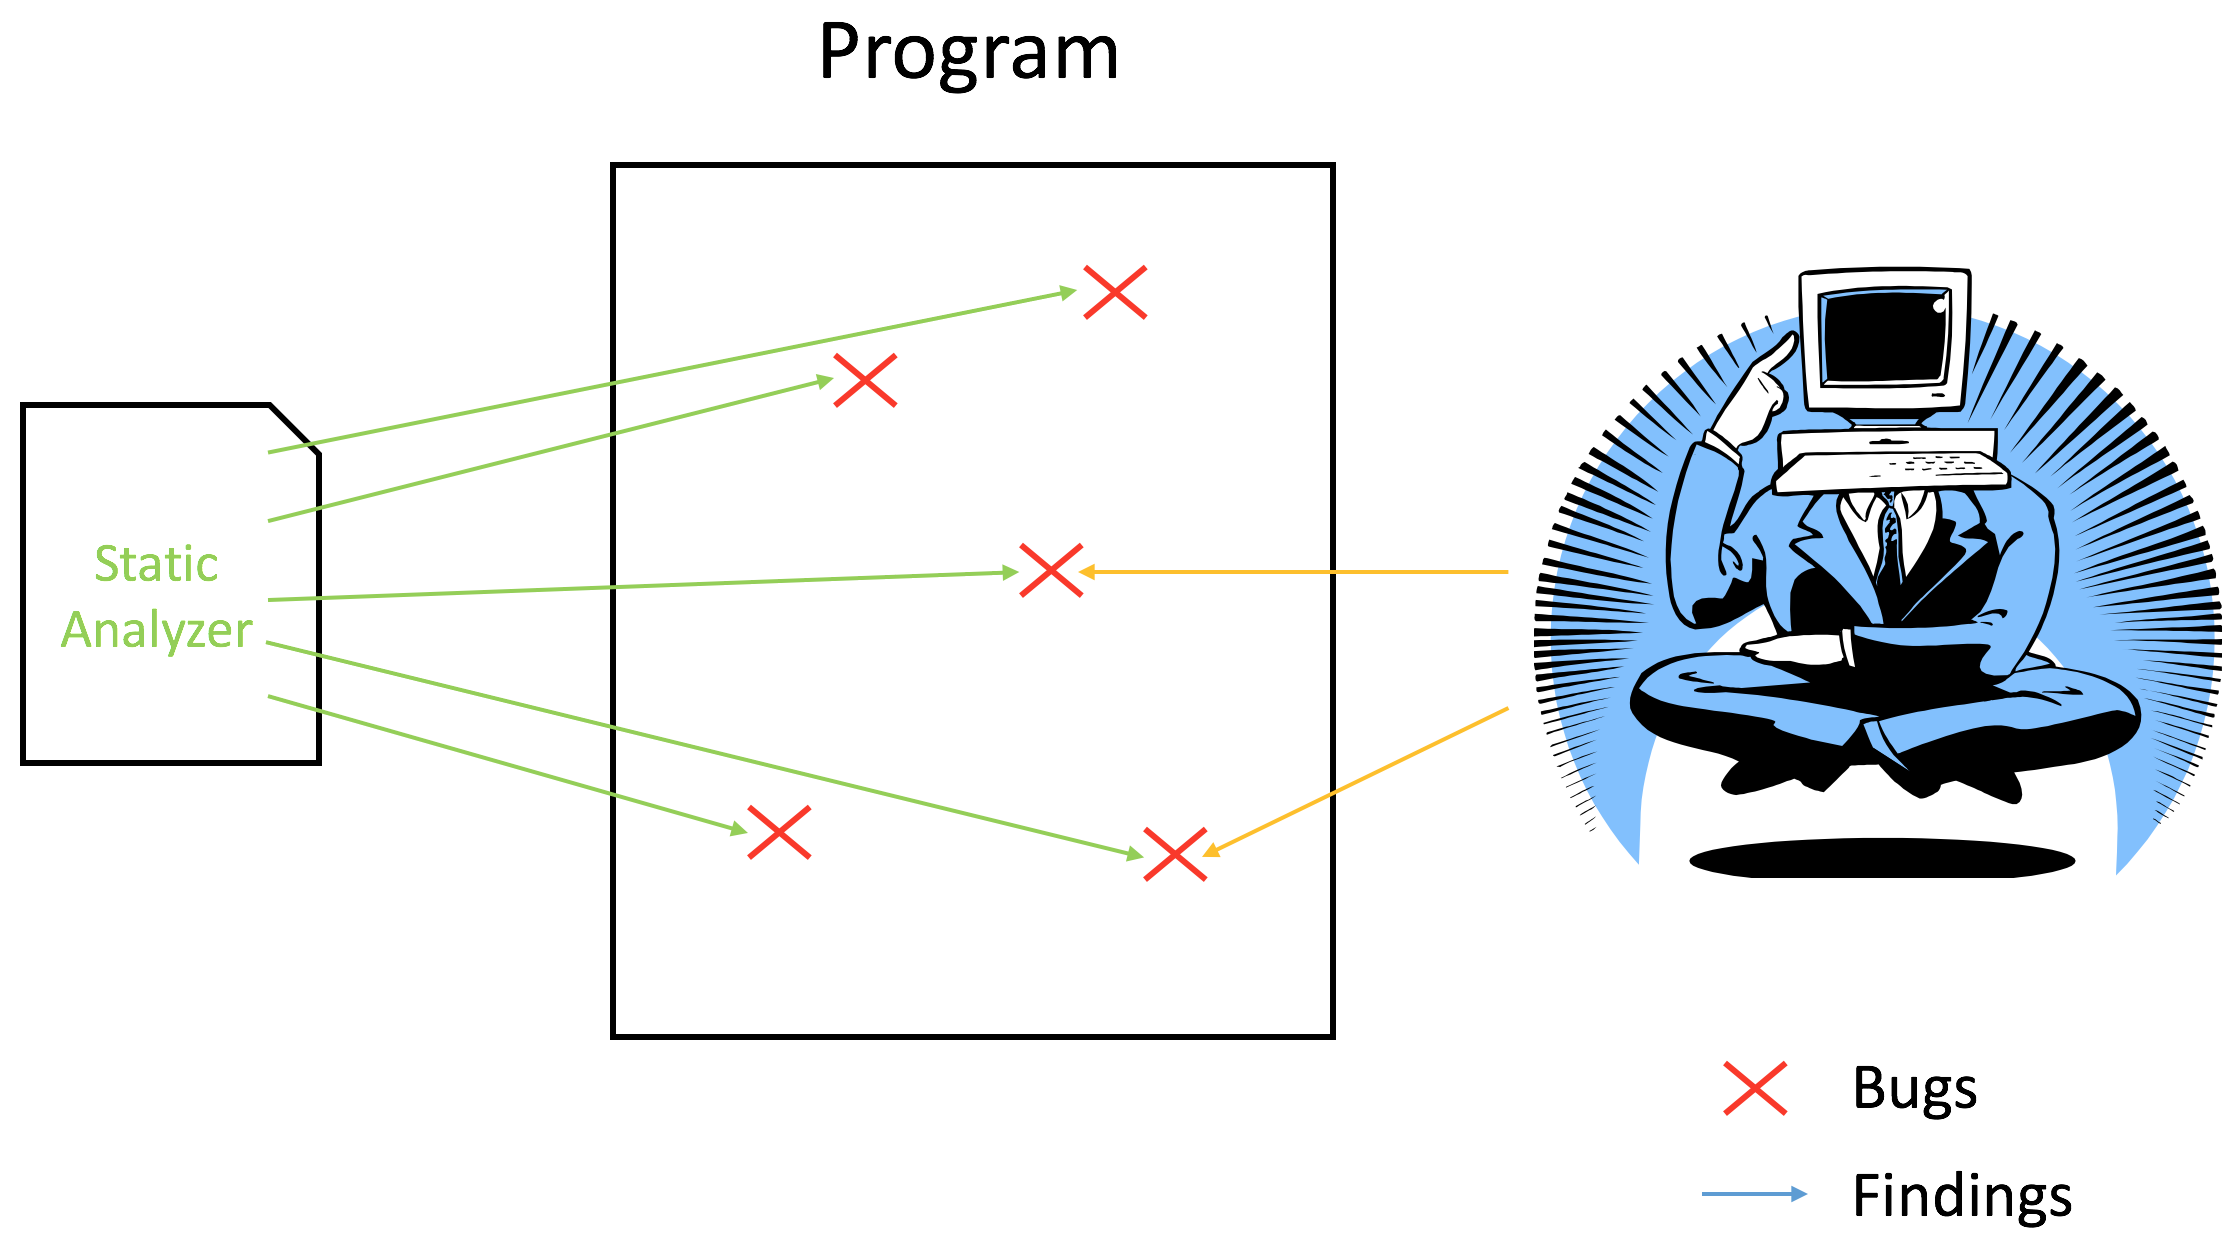
\includegraphics[scale=0.3]{figures/the-dream}
      \caption{The Dream of Every Developer}
    \end{figure}
  \end{frame}

  \begin{frame}{Problem solved! Ugh\ldots{} not quite!}
    \begin{figure}
      \centering
      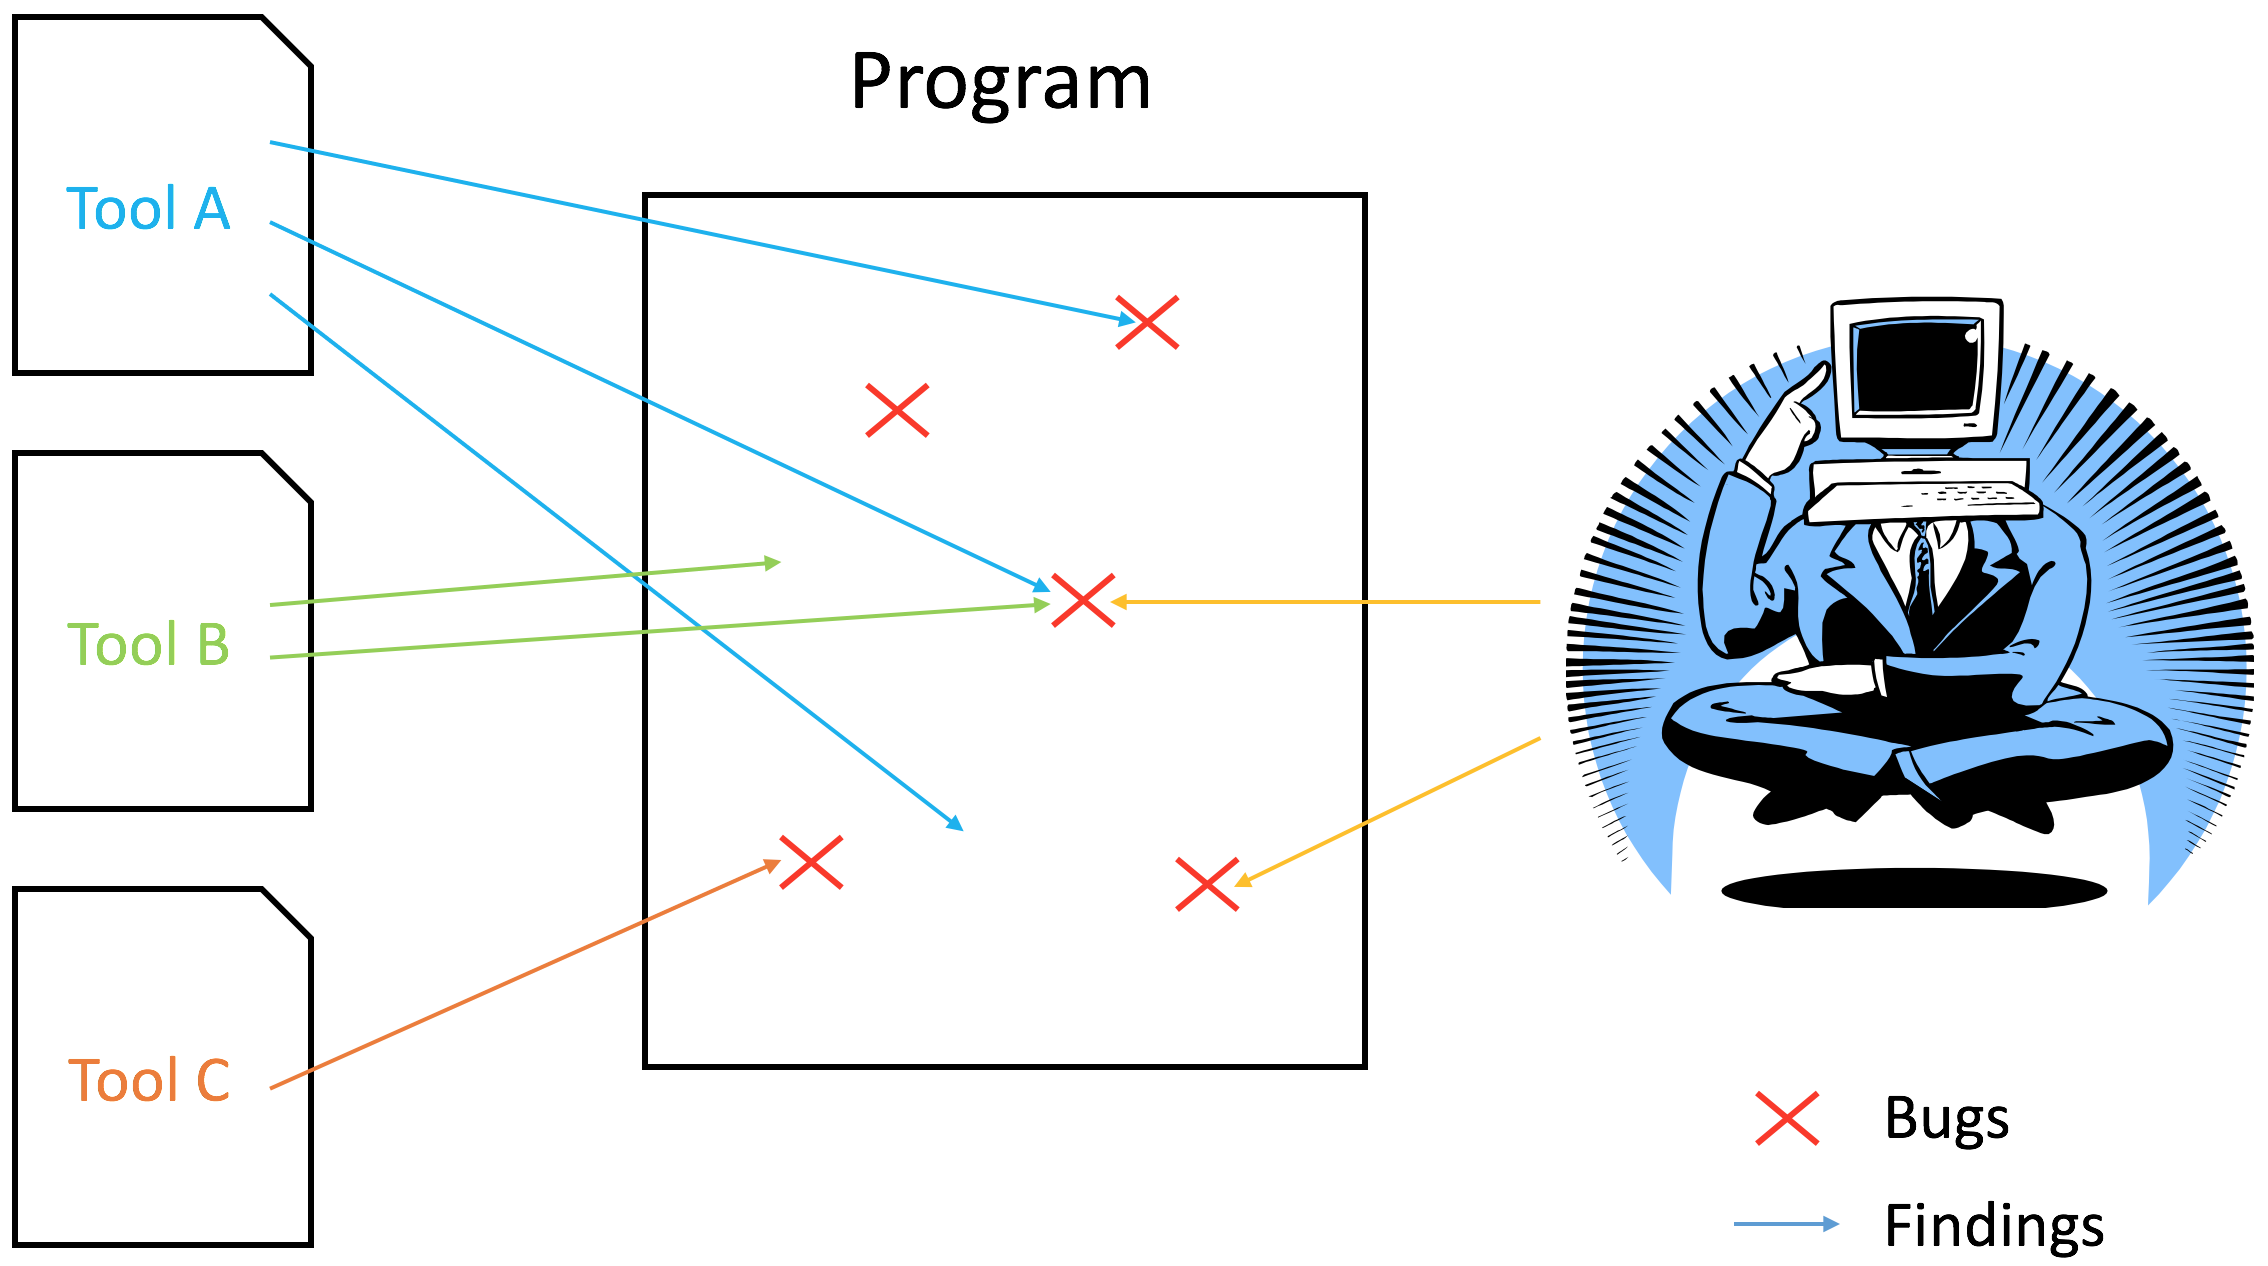
\includegraphics[scale=0.3]{figures/static-analyzers}
      \caption{Static Analyzers Imperfections}
    \end{figure}
  \end{frame}
    
  \subsection{Static Analysis Tool Exposition (SATE) Project}

  \begin{frame}{Static Analysis Tool Exposition (SATE)}
    \textbf{Goal:} \alert{Evaluate the performance of static analyzers}\\
    \pause
    \vfill
    \textbf{Process:}
    \begin{enumerate}
    \item Provide tool makers with \textbf{test suites}
    \item Tool makers run their static analyzers and generate reports
    \item SAMATE team analyzes the reports
    \end{enumerate}
    \pause
    \vfill
    \begin{block}{Definitions}
      \vspace{0.3em}
      A \textcolor{mLightGreen}{test suite} is a set of \textbf{test cases}.\\
      \pause
      \vspace{0.3em}
      A \textcolor{mLightGreen}{test case} is a program with bugs.
    \end{block}
  \end{frame}

  \begin{frame}{Desired Characteristics of Test Suites}
    \begin{figure}
      \centering
      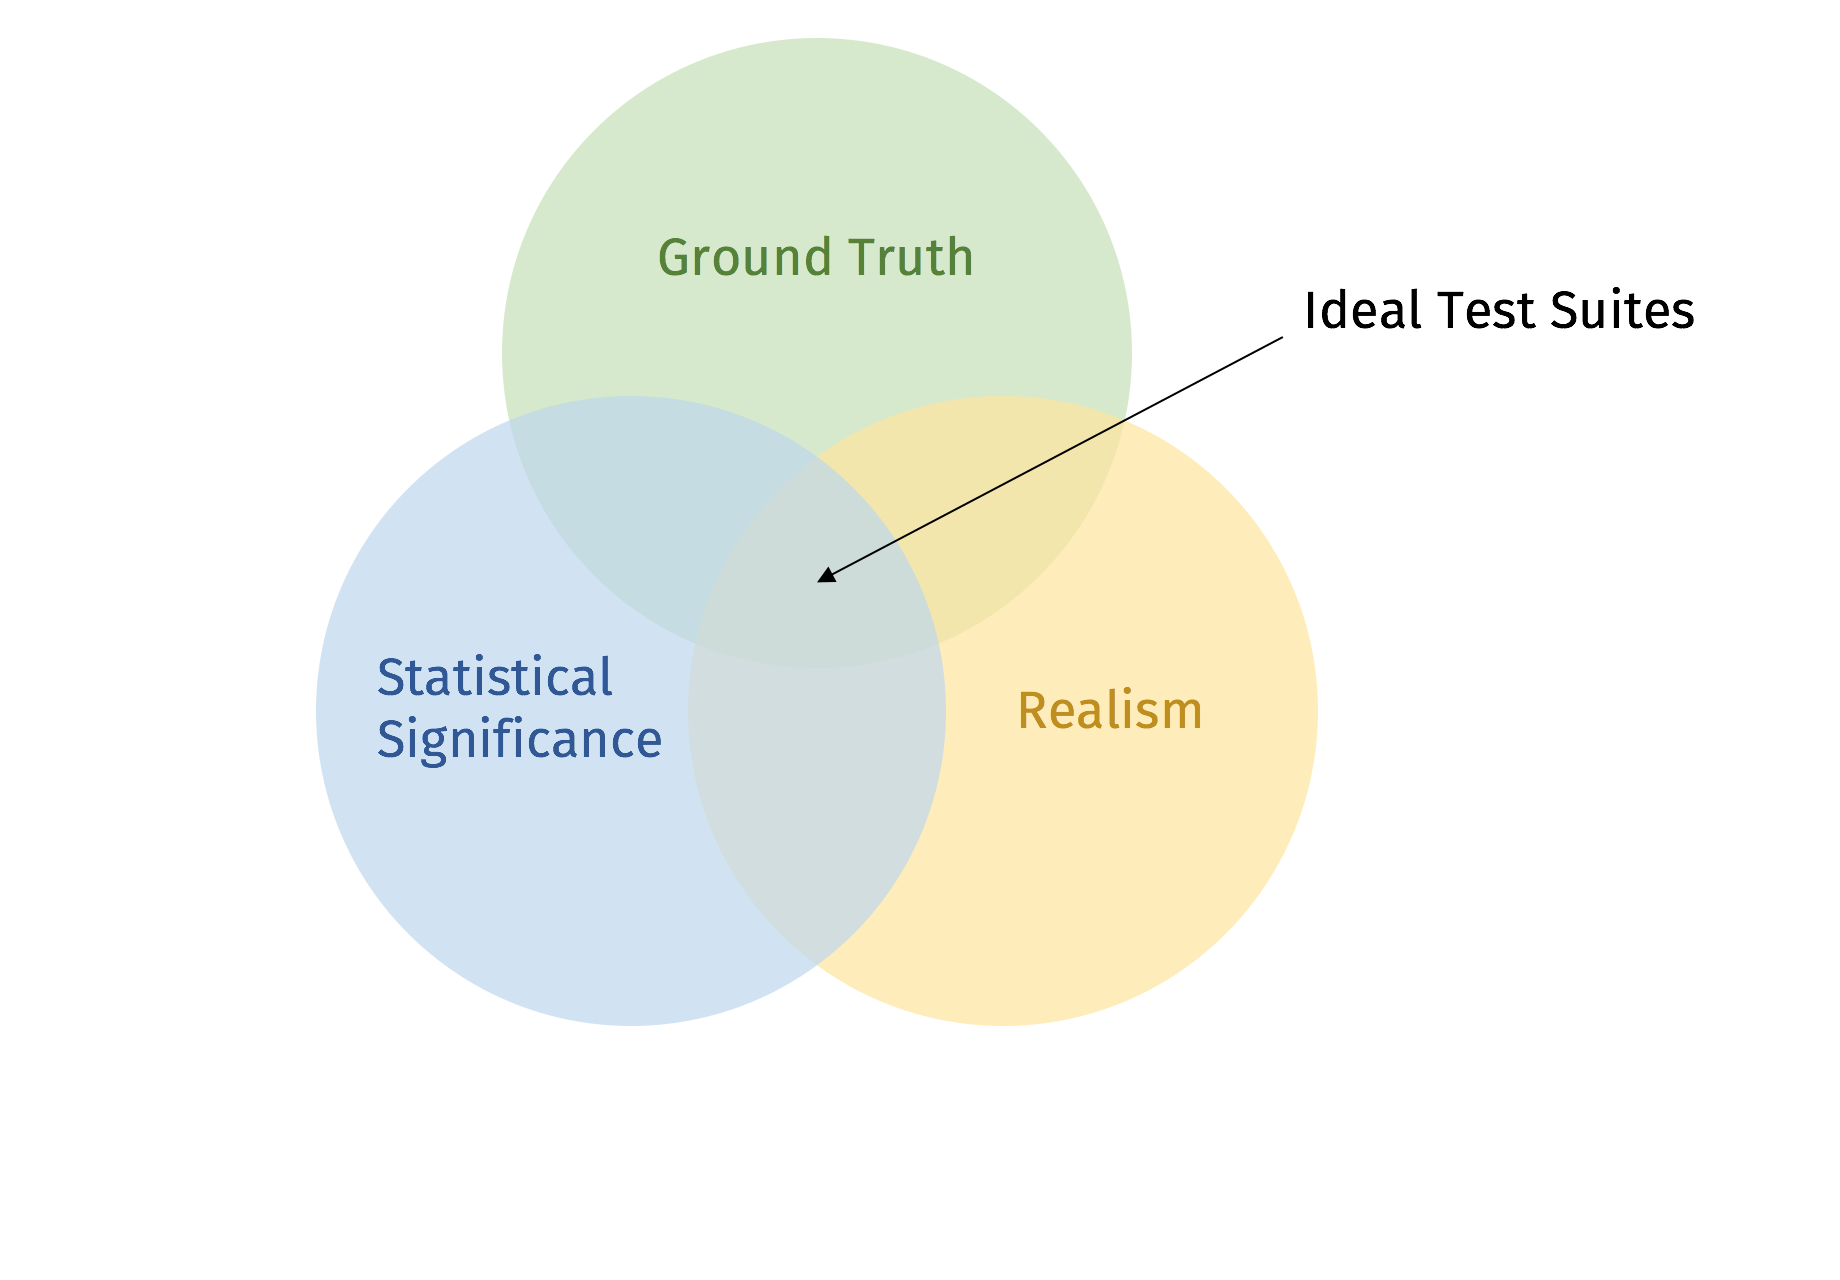
\includegraphics[scale=0.3]{figures/ideal-test-suites}
      \caption{Ideal Test Suites}
    \end{figure}
  \end{frame}

  \begin{frame}{SATE V Test Suites}
    \begin{figure}
      \centering
      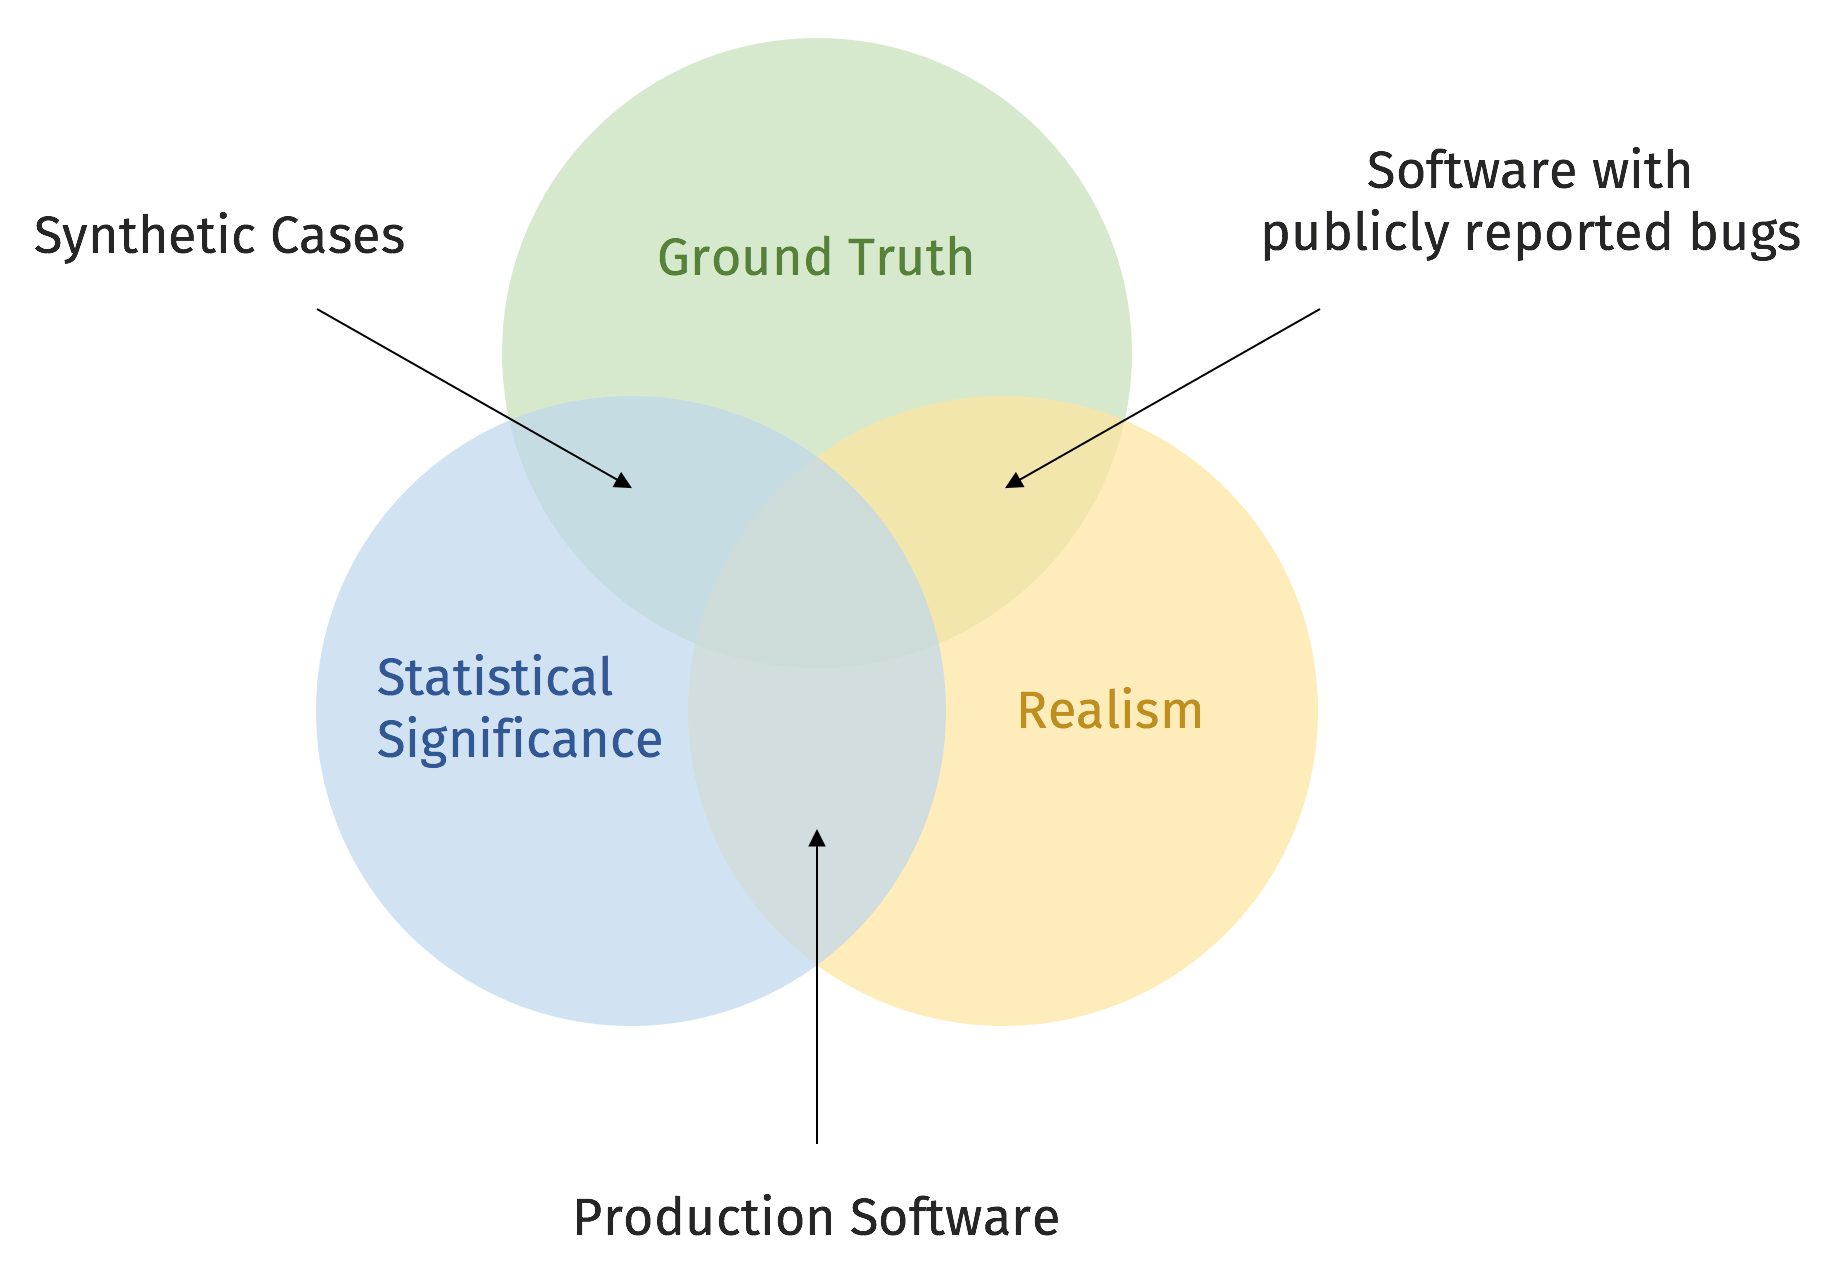
\includegraphics[scale=0.3]{figures/sate-v-test-suites}
      \caption{SATE V Solution}
    \end{figure}
  \end{frame}
  % End of section
  
  % Beginning of section
  \section{SATE VI Test Case Development}

  \subsection{Challenges and Goals}

  \begin{frame}{Project Goals}
    \begin{itemize}
    \setlength\itemsep{1em}
    \item Produce 2 test suites, a \textbf{C/C++ track}, and a \textbf{Java track}
    \pause
    \item The test suites must present the following characteristics:
      \vspace{0.3em}
      \begin{itemize}
      \setlength\itemsep{0.5em}
      \item \textbf{Ground Truth} $\rightarrow$ We know where the bugs are
      \item \textbf{Realism} $\rightarrow$ As close as possible to industrial software
      \item \textbf{Statistical Significance} $\rightarrow$ We want a lot of bugs, hundreds of them!
      \end{itemize}
    \pause
    \item A \textbf{large spectrum of bug types}
    \end{itemize}
  \end{frame}

  \begin{frame}{Project Challenges}
    \begin{block}{Challenge \#1:}
      No such test case exists in nature
    \end{block}
    \pause
    \begin{block}{Challenge \#2:}
      Developing test cases from scratch is not an option
    \end{block}
    \pause
    \vspace{1.5em}
    \centering
    \begin{LARGE}
      What about modifying existing source code then?\\ And \alert{insert bugs} in it?!
    \end{LARGE}
  \end{frame}

  \begin{frame}{Project Challenges}
    Injecting bugs into existing source code \ldots{} is that hard?\\
    \pause
    \begin{itemize}
    \setlength\itemsep{0.4em}
    \item Getting to know an existing project is \textbf{insanely time consuming}
    \pause
    \item How would we \textbf{identify vulnerable source code locations} to inject bugs?
    \pause
    \item Realism VS. Modifying the program's behavior
    \pause
    \item Different bug types, different processes?
    \pause
    \item Ability to \textbf{trigger the bugs}?
    \end{itemize}
    \pause
    \vspace{0.5em}
    $\rightarrow$ Challenging task and really {\LARGE\alert{time consuming}} task when done manually
  \end{frame}
  
  \subsection{Opportunities with Automated Bug Injection Techniques}

  \begin{frame}{Automated Bug Injection Techniques}
    Some automated bug injection techniques are starting to emerge:
    \begin{itemize}
    \item Automating a \textbf{code mutation} process
    \item Injecting small snippets of flawed code (STONESOUP)
    \item Analyzing the control flow and data flow (LAVA)
    \end{itemize}
    \pause
    Some of those techniques are \alert{powerful}, but they all lack one thing \ldots{}
    \pause
    \begin{center}
      \begin{large}
        \textbf{The crafted bugs are not realistic enough yet}
      \end{large}
    \end{center}
  \end{frame} 

  \begin{frame}{About Combining Both Worlds}
    \centering
    \begin{table}
    \begin{tabular}{lcc}
      \toprule
      & Manual Injection & Automated Injection \\
      \midrule
      Programming Languages & \textcolor{custom-green}{\ding{51}} & \textcolor{custom-red}{\ding{55}} \\
      \midrule
      Ground Truth & \textcolor{custom-green}{\ding{51}} & \textcolor{custom-green}{\ding{51}} \\
      \midrule
      Realism & \textcolor{custom-green}{\ding{51}} & \textcolor{custom-red}{\ding{55}} \\
      \midrule
      Statistical Significance & \textcolor{custom-red}{\ding{55}} & \textcolor{custom-green}{\ding{51}} \\
      \midrule
      Bug Spectrum & \textcolor{custom-green}{\ding{51}} & \textcolor{custom-red}{\ding{55}} \\
      \bottomrule
    \end{tabular}
    \caption{Manual Bug Injection VS. Automated Bug Injection}
    \end{table}
    \pause
    \textbf{Automating part of the process would get us the best of both worlds.}
  \end{frame}
  
  \subsection{Project Plan}
  \begin{frame}{My Action Plan}
    \begin{enumerate}
      \setlength\itemsep{1em}
      \item Bug injection \textbf{state of the art}
      \pause
      \item \textbf{Get familiar} with the chosen technique
      \pause
      \item \textbf{Use it} on potential future test cases
      \pause
      \item Speed the process of \textbf{manual bug injection}
      \pause
      \item \textbf{Design a process} to produce test suites for SATE VI
    \end{enumerate}
  \end{frame}
  % End of section

  % Beginning of section
  \section{A Focus on LAVA, a Large-scale and Automated Vulnerability Addition Tool}

  \begin{frame}{LAVA Software}
    \begin{columns}
      \begin{column}{0.25\textwidth}
        \begin{figure}
          \centering
          \hspace{1em}
          
\includegraphics[scale=0.35]{figures/lava-logo}
          \caption{LAVA Logo}
        \end{figure}
      \end{column}
      \begin{column}{0.75\textwidth}
        \begin{itemize}
        \setlength\itemsep{1em}
        \item \textbf{L}arge-scale \textbf{A}utomated \textbf{V}ulnerability \textbf{A}ddition tool
        \item Developed by the MIT Lincoln Laboratory and the University of New York
        \item \textbf{Motivation:} ``Generate \alert{large ground-truth vulnerability corpora} to enable rigorous tool evaluation''
        \item \textbf{How?} Inject bugs into existing C programs by analyzing the \alert{control flow} and \alert{data flow}
        \end{itemize}
      \end{column}
    \end{columns}
  \end{frame}
  
  \subsection{LAVA Process Overview}

  \begin{frame}{Desired Bugs Characteristics}
    LAVA was implemented with the following requirements in mind. Bugs should:
    \begin{itemize}
    \setlength\itemsep{1em}
    \item[\textcolor{custom-green}{\ding{51}}] Be \textbf{cheap} and \textbf{plentiful}
    \item[\textcolor{custom-green}{\ding{51}}] Span the execution lifetime of a program
    \item[\textcolor{custom-green}{\ding{51}}] Be embedded in representative control and data flow
    \item[\textcolor{custom-green}{\ding{51}}] Come with an input that serves as a \textbf{proof of existence}
    \item[\textcolor{custom-green}{\ding{51}}] Manifest for a very small fraction of possible inputs
    \end{itemize}
  \end{frame}

  \begin{frame}{DUAs and ATPs}
    \vspace{0.5em}
    \begin{definition}
      \vspace{0.3em}
      \textcolor{mLightGreen}{DUA} stands for \textbf{D}ead \textbf{U}ncomplicated and \textbf{A}vailable data.\\
      \vspace{-0.2em}
      \begin{description}[Uncomplicated]
        \item[Dead] Qualifies data that does \alert{not influence the program's behavior}
        \item[Uncomplicated] The data is \alert{not altered much} so we can easily control its value 
        \item[Available] The data should be \alert{accessible} via program variables
      \end{description}
    \end{definition}
    \pause
    \begin{definition}
      \vspace{0.3em}
      \textcolor{mLightGreen}{ATP} stands for \textbf{AT}tack \textbf{P}oints.\\
      \vspace{0.3em}
      An ATP is a \textbf{site} in the source code, a location, where identifiable structure makes it a \alert{potential place to inject a bug}.
    \end{definition}
  \end{frame}

  \begin{frame}{LAVA Bug Formula}
    \begin{enumerate}
    \item Find the DUAs and ATPs in the program
    \item Make the DUAs available at the ATPs
    \item Inject bugs by using DUAs with altered values at the ATPs
    \end{enumerate}
    \begin{figure}
      \centering
      
\includegraphics[scale=0.3]{figures/lava-bug}
      \caption{LAVA Bug Formula: DUAs + ATPs}
    \end{figure}
  \end{frame}

  \begin{frame}{Why Should We Use LAVA?}
    \begin{table}
      \begin{tabular}{ll}
        \toprule
        \multicolumn{2}{c}{LAVA or not LAVA?}\\
        \midrule
        \multicolumn{1}{c}{\textcolor{custom-green}{Pros}} & \multicolumn{1}{c}{\textcolor{custom-red}{Cons}} \\
        \midrule
        \textcolor{custom-green}{\ding{51}} Inject a lot of bugs & \textcolor{custom-red}{\ding{55}} Works only for C Programs \\
        \textcolor{custom-green}{\ding{51}} The most sophisticated so far & \textcolor{custom-red}{\ding{55}} Addresses a single bug type \\
        \textcolor{custom-green}{\ding{51}} Very fast method & \textcolor{custom-red}{\ding{55}} Bugs not realistic enough \\
        \textcolor{custom-green}{\ding{51}} Hope to extend it & \textcolor{custom-red}{\ding{55}} Proof of concept more than a real product \\
        \textcolor{custom-green}{\ding{51}} Access to the DUAs and ATPs & \\
        \bottomrule
      \end{tabular}
      \caption{Advantages and Disadvantages of Using LAVA}
    \end{table}
  \end{frame}
  
  \subsection{Using LAVA on Real Code}

  \begin{frame}{Running LAVA}
    Tried to run LAVA on two programs:
    \begin{itemize}
    \item \textit{File} $\rightarrow$ \textcolor{custom-green}{Successful}
    \item \textit{Hping} $\rightarrow$ \textcolor{custom-red}{A real pain \ldots}
    \end{itemize}
    \pause
    \vspace{0.5em}
    \textbf{Poor documentation} \\
    \vspace{0.3em}
    LAVA expects the software to be \textbf{compliant with the GNU build system} \\
    \vspace{0.3em}
    The system architecture is \textbf{really complex}.
  \end{frame}

  \subsection{Extending LAVA}

  \begin{frame}{Extending LAVA}
    Some things I have done so far to improve LAVA:
    \begin{itemize}
    \setlength\itemsep{1em}
    \item Improved the \textbf{LAVA configuration system}
    \item Submitted changes to the LAVA team:
      \begin{itemize}
        \item \textbf{Fixed} bugs
        \item \textbf{Refactored} duplicated source code into functions
        \item \textbf{Implemented} new features
      \end{itemize}
      All were \textcolor{custom-green}{accepted}!
    \item Designed an SQL query to \alert{use the LAVA database information}
    \end{itemize}
  \end{frame}

  \begin{frame}{Using DUAs and ATPs to manually inject vulnerabilities}
    \begin{figure}
      \centering
      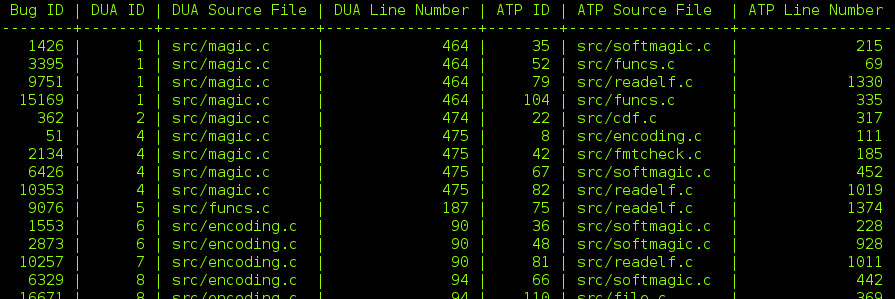
\includegraphics[scale=0.43]{figures/sql-output}
      \caption{SQL Request Output on LAVA Database}
    \end{figure}
  \end{frame}
  % End of section

  % Beginning of section
  \section*{Conclusion}

  \begin{frame}{Project Results}
    \begin{enumerate}
      \setlength\itemsep{1em}
      \item[\textcolor{custom-green}{\ding{51}}] Bug injection state of the art
      \pause
      \item[\textcolor{custom-green}{\ding{51}}] Get familiar with the chosen technique
      \pause
      \item[\textcolor{mLightBrown}{\ding{51}}] Use it on potential future test cases
      \pause
      \item[\textcolor{custom-green}{\ding{51}}] Speed the process of manual bug injection
      \pause
      \item[\textcolor{custom-red}{\ding{55}}] Design a process to produce test suites
    \end{enumerate}
  \end{frame}

  \begin{frame}{Future Work}
    On the short-term, for SATE VI:
    \begin{itemize}
    \item[\ding{43}] Run LAVA on other test cases
    \item[\ding{43}] Insert bugs in a semi-automated way using LAVA
    \item[\ding{43}] JAVA test suite (STONESOUP?)
    \end{itemize}
    \pause
    On the long-term:
    \begin{itemize}
    \item[\ding{43}] Extend LAVA to find new ATPs
    \item[\ding{43}] Or \ldots{} build our own product?
    \end{itemize}
  \end{frame}
  
  % End of section
  
  \begin{frame}[standout]
    \begin{huge}
      Thank you for your attention!\\\alert{Questions?\\}
    \end{huge}
    \vspace{2.5em}
    \begin{scriptsize}
      For any follow-up, feel free to contact me at\\
      damien.cupif@nist.gov
    \end{scriptsize}
  \end{frame}

  \end{document}
